% =====================================================================
% AI Academy -- National AI Center
% Software Engineering Final Project -- Team Report
% Topic 4: Async Research Assistant
% Compile with pdfLaTeX (or Overleaf).
% =====================================================================

\documentclass[11pt,a4paper]{article}

\usepackage[dvipsnames]{xcolor}
\definecolor{accent2}{HTML}{8B0000}
\definecolor{ph}{HTML}{6B7280}

% ===== CONFIGURATION =================================================
\newcommand{\teamname}{Topic Four}
\newcommand{\topicchoice}{Topic 4 -- Async Research Assistant}
\newcommand{\member}[2]{\textbf{#1} (#2)}
\newcommand{\reportdate}{September 18, 2026}
\newcommand{\repolink}{\texttt{github.com/nuralnetworks/async-research-assistant}}

% ===== course meta ===================================================
\newcommand{\coursecode}{AI-ENG-110}
\newcommand{\coursename}{Software Engineering}
\newcommand{\institution}{AI Academy, National AI Center}
\newcommand{\semester}{Spring 2026}

% ===== PACKAGES ======================================================
\usepackage[margin=2.2cm,headheight=15pt]{geometry}
\usepackage[T1]{fontenc}
\usepackage[utf8]{inputenc}
\usepackage[final,protrusion=true,expansion=false]{microtype}
\usepackage{amsmath,amssymb}
\usepackage{graphicx}
\usepackage{booktabs}
\usepackage{array}
\usepackage{tabularx}
\usepackage{ragged2e}
\usepackage{enumitem}
\usepackage[parfill]{parskip}
\usepackage{listings}
\usepackage[most]{tcolorbox}
\usepackage{titlesec}
\usepackage{fancyhdr}
\usepackage{lastpage}
\usepackage{tikz}
\usetikzlibrary{arrows.meta,positioning}
\usepackage[hidelinks]{hyperref}

\emergencystretch=3em
\hbadness=10000
\hfuzz=2pt

\hypersetup{
  colorlinks=true,
  linkcolor=NavyBlue,
  urlcolor=NavyBlue,
  citecolor=NavyBlue,
  pdftitle={\coursecode\ Final Project Report},
  pdfauthor={\teamname}
}

% ===== STYLING =======================================================
\definecolor{accent}{HTML}{0B3D91}
\definecolor{soft}{HTML}{F2F4F8}

\titleformat{\section}
  {\Large\bfseries\color{accent}}{\thesection.}{0.6em}{}
\titleformat{\subsection}
  {\large\bfseries\color{accent}}{\thesubsection}{0.5em}{}

\definecolor{codegreen}{rgb}{0,0.55,0}
\definecolor{codegray}{rgb}{0.4,0.4,0.4}
\definecolor{codepurple}{rgb}{0.55,0,0.78}
\definecolor{backcolour}{rgb}{0.97,0.97,0.97}

\lstdefinestyle{python}{
  language=Python,
  backgroundcolor=\color{backcolour},
  commentstyle=\color{codegreen},
  keywordstyle=\color{accent},
  numberstyle=\tiny\color{codegray},
  stringstyle=\color{codepurple},
  basicstyle=\ttfamily\footnotesize,
  breakatwhitespace=false,
  breaklines=true,
  keepspaces=true,
  numbers=left,
  numbersep=6pt,
  tabsize=2,
  frame=single,
  framerule=0.4pt,
  rulecolor=\color{black!30},
}

\pagestyle{fancy}
\fancyhf{}
\fancyhead[L]{\small\textit{\coursecode\ -- Final Report -- \teamname}}
\fancyhead[R]{\small\textit{\semester}}
\fancyfoot[L]{\small\textit{\institution}}
\fancyfoot[R]{\small Page \thepage\ of \pageref{LastPage}}
\renewcommand{\headrulewidth}{0.4pt}
\renewcommand{\footrulewidth}{0.4pt}

% =====================================================================
\begin{document}

\begin{center}
{\small \textsc{\institution} \\[0.2em] \textsc{\coursecode\ -- \coursename\ -- \semester}}\\[1.2em]
{\Large\bfseries\color{accent} Final Project Report}\\[0.3em]
{\LARGE\bfseries \topicchoice}\\[0.6em]
\rule{0.85\textwidth}{0.6pt}
\end{center}

\vspace{0.6em}
\begin{tabularx}{\textwidth}{@{}lXlX@{}}
\textbf{Team:} & \teamname & \textbf{Date:} & \reportdate \\
\textbf{Repo:} & \repolink \\
\end{tabularx}

\noindent\begin{tabularx}{\textwidth}{@{}lX@{}}
\textbf{Members:} & \member{Nural Shukurlu}{@nuralnetworks},\quad
  \member{Emil Mammadov}{@Emilsdeyta} \\
 & \member{Mahammadali Babayev}{@mahammadalibabayev11},\quad
  \member{Bailar Bayramov}{@bailar-dev} \\
\end{tabularx}
\vspace{0.4em}\hrule\vspace{0.6em}

% ===== EXECUTIVE SUMMARY =============================================
\section*{Executive Summary}
\addcontentsline{toc}{section}{Executive Summary}

We built a research assistant that takes a plain question, queries Wikipedia, arXiv, and web search at the same time, and returns one short answer with numbered citations. Fetching the three sources concurrently instead of one after another cut a 15-fetch benchmark from 4.52\,s to 2.73\,s on our machine. The most valuable robustness work was not the retry logic but the cache: we found empty upstream responses being stored as valid results and served for a full day, and fixed it by never caching empties and versioning cache keys. The surprise of the project was how much behavior lives outside our code: Wikipedia rejects long questions and the default HTTP client, arXiv moved behind a redirect, and DuckDuckGo throttles whole networks, so a large part of ``robustness'' turned out to be shaping requests the providers accept. If we started over, we would write the failure-injection tests before the happy paths, because every real bug we met came from a provider, not from our logic.

\tableofcontents
\vspace{0.6em}\hrule\vspace{0.4em}

% =====================================================================
\section{Project Overview}

\subsection{Problem framing \& scope}

A user asks a research question in plain language, for example ``What is photosynthesis and what are its main stages?'' Our system queries three public sources in parallel (Wikipedia for encyclopedic summaries, arXiv for papers, web search for everything else), then asks a language model to write a 3--6 sentence answer that cites the retrieved excerpts by number. The input is one string; the output is the answer text plus a reference list of titles and URLs, printed to the terminal or as JSON.

We expose three commands under \texttt{python -m researcher}: \texttt{ask} for one question, \texttt{demo} for the five sample questions, and \texttt{bench} for the timing comparison. Each command also accepts \texttt{--offline}, which swaps the network and the LLM for canned fakes so the whole pipeline runs with no keys and no network. We use Gemini for synthesis (the exact model id lives in \texttt{.env}, so it can change without touching code) and Tavily for live web search,
with DuckDuckGo as the keyless default.

We deliberately did not build the HTTP API the brief suggests for other topics, since Topic~4 requires only a CLI, and we did not build multi-provider failover: one well-wrapped provider per slot beat two half-wrapped ones in the time we had. We tightened the brief in one place the graders will notice: the spec asks for caching by \texttt{(source, query)}, and we additionally version cache keys and refuse to cache empty hits, because we watched stale empties poison answers for a full TTL window.

\subsection{Provider choice and the AI module contract}

For synthesis we use Google Gemini, because its free tier covered our whole demo budget (all five sample questions cost a fraction of a cent) and its Python SDK needed no extra services. For web search we default to DuckDuckGo since it needs no key, and use Tavily (free tier) whenever a key is present, because its result quality is clearly higher. Wikipedia and arXiv need no keys at all. We call exactly four functions from the provided package: \texttt{ai.fetch\_wikipedia}, \texttt{ai.fetch\_arxiv}, \texttt{ai.fetch\_web}, and \texttt{ai.synthesize}. We did not modify the public interface of the provided \texttt{ai/} package in any way; a file-by-file diff against the distributed folder shows no differences in any \texttt{.py} file.

A malformed model response never reaches our output unexamined. The provided \texttt{synthesize} already drops out-of-range citation indices, and on top of that our wrapper rejects empty answers as provider errors (retried, then surfaced), validates question length before calling, and requires a non-empty source list. Semantically wrong but well-formed output, for example an answer that ignores the sources, is handled the way the topic intends: the synthesizer prompt constrains the model to the numbered sources, and our demo runs showed the model saying plainly when sources lack the answer instead of inventing one.

% =====================================================================
\section{Architecture}\label{sec:arch}

\subsection{Module map}

\begin{center}
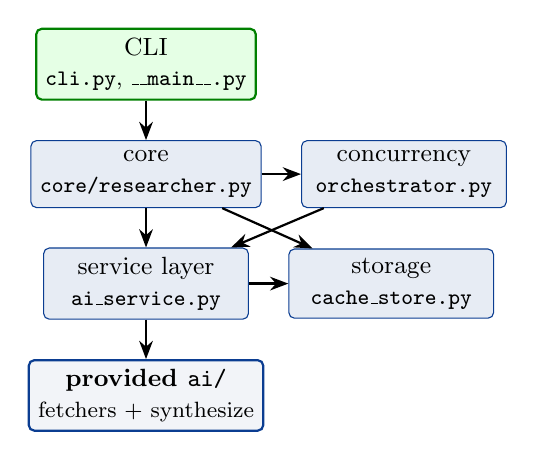
\begin{tikzpicture}[
  node distance=5mm,
  box/.style={draw,rounded corners=2pt,minimum width=2.6cm,minimum height=0.85cm,align=center,font=\small},
  aibox/.style={box,fill=soft,draw=accent,thick},
  sebox/.style={box,fill=accent!10,draw=accent},
  entry/.style={box,fill=green!10,draw=green!50!black,thick},
  arrow/.style={-Stealth,thick}
]
  \node[entry] (cli) {CLI\\{\footnotesize\texttt{cli.py}, \texttt{\_\_main\_\_.py}}};
  \node[sebox,below=of cli] (core) {core\\{\footnotesize\texttt{core/researcher.py}}};
  \node[sebox,right=of core] (conc) {concurrency\\{\footnotesize\texttt{orchestrator.py}}};
  \node[sebox,below=of core] (svc) {service layer\\{\footnotesize\texttt{ai\_service.py}}};
  \node[sebox,right=of svc] (store) {storage\\{\footnotesize\texttt{cache\_store.py}}};
  \node[aibox,below=of svc] (ai) {\textbf{provided \texttt{ai/}}\\{\footnotesize fetchers + synthesize}};
  \draw[arrow] (cli) -- (core);
  \draw[arrow] (core) -- (conc);
  \draw[arrow] (core) -- (svc);
  \draw[arrow] (conc) -- (svc);
  \draw[arrow] (svc) -- (ai);
  \draw[arrow] (svc) -- (store);
  \draw[arrow] (core) -- (store);
\end{tikzpicture}
\end{center}

Only \texttt{services/ai\_service.py} crosses the \texttt{ai/} boundary, so swapping Anthropic for OpenAI touches exactly one file (plus \texttt{.env}). Only the service and the core cross the storage boundary, through the \texttt{CacheStore} interface, so SQLite could be replaced without touching fetch or CLI code.

Module by module: \texttt{config.py} reads the environment into a frozen \texttt{Settings} object every module imports. \texttt{models.py} holds the request/result pydantic models. \texttt{services/ai\_service.py} wraps each \texttt{ai.*} call with cache, rate limiting, retries, timeouts, and logging. \texttt{services/rate\_limit.py} is a token bucket guarding external calls. \texttt{storage/cache\_store.py} persists per-source results and query history in SQLite with a file-based fallback. \texttt{concurrency/orchestrator.py} runs the three fetches together with per-source timeouts. \texttt{core/researcher.py} validates, orchestrates, synthesizes, and persists. \texttt{cli.py} parses arguments and renders answers.

\subsection{OOP design \& key abstractions}

Our inheritance example is the cache backend, and our composition example is the service that uses it:

\begin{lstlisting}[style=python]
class CacheStore(ABC):
    def get(self, source: str, query: str) -> list[Source] | None: ...
    def set(self, source: str, query: str, value: list[Source]) -> None: ...
    def clear(self) -> None: ...

class SqliteCacheStore(CacheStore): ...    # main store
class FileJsonCacheStore(CacheStore): ...  # fallback under CACHE_DIR

class ResilientAIService:  # uses a store, is not a store
    def __init__(self, settings: Settings, cache: CacheLike,
                 limiter: RateLimiter) -> None: ...
\end{lstlisting}

We chose an ABC for the store because the two backends share lifecycle and error-handling expectations that a bare callable cannot express, and because tests substitute fakes with identical shapes. We chose composition for the service deliberately: a service \emph{uses} a cache and a limiter, it is not a kind of either, and inheritance there would have welded retry policy to storage details. The rate limiter mirrors the same split with its own small ABC plus a no-op implementation for offline runs and tests.

\subsection{Data flow across module boundaries}

Our own models are \texttt{ResearchRequest} (question, source subset, cache flag, per-query limit), \texttt{SourceFailure} (source plus error text), \texttt{ResearchResult} (answer, citations, sources, failures, timings, cache flag, warnings), and \texttt{FetchOutcome} (the orchestrator's internal result). We reuse the provided \texttt{Source}, \texttt{Citation}, and \texttt{AnswerWithCitations} directly instead of wrapping them, because they already forbid extra fields and freeze mutation, which is exactly what we want crossing into synthesis. No naked dictionaries cross any module boundary; the one place raw JSON appears is inside the SQLite payload column, which is an implementation detail of the store, never an interface.

% =====================================================================
\section{Concurrency \& Performance}\label{sec:concurrency}

\subsection{Why this concurrency model}

We used \texttt{asyncio} with a single shared \texttt{httpx.AsyncClient} and \texttt{asyncio.gather(return\_exceptions=True)}. The workload is three independent network calls per question, so the bottleneck is waiting on providers, which is what async I/O parallelizes best. Threads would add GIL-era complexity for zero gain here, and processes would be absurd for HTTP waits. Parallelism is bounded by a semaphore set from \texttt{MAX\_PARALLEL} (5 in production settings, 3 inside the bench harness), picked so a burst of questions cannot draw 429 responses from polite public APIs. With the bound at 1 the pipeline degrades to sequential; at 100 the providers throttle us, which we verified the painful way against arXiv during development. Since a single source round trip costs hundreds of milliseconds, even two sources finish faster together; the gather overhead itself is noise next to any real network call.

\subsection{Sequential-vs-concurrent benchmark}

\begin{center}\small
\begin{tabular}{lcccc}
\toprule
\textbf{Workload} & $N$ & \textbf{Sequential (s)} & \textbf{Concurrent (s)} & \textbf{Speedup} \\
\midrule
5 questions $\times$ 3 sources & 15 fetches & 4.52 & 2.73 & 1.66$\times$ \\
\bottomrule
\end{tabular}
\end{center}

Measured on Windows with Python 3.13.3 and a cleared cache via \texttt{python scripts/bench.py --offline} (reproduced in the README; CI runs Python 3.12). Each simulated fetch sleeps 300\,ms, so the theoretical ceiling for 15 fetches is far above what we reached. The new bottleneck is our own per-process token bucket plus the single synthesis call that stays serial by nature. Pushing further would mean a higher bucket rate against paid provider tiers, which we did not have.

\subsection{Rate limit \& politeness}

We use a token-bucket limiter (\texttt{rate\_per\_sec}, \texttt{capacity} both derived from \texttt{MAX\_PARALLEL}) checked before every external call, plus tenacity backoff on 429/5xx inside the wrapper. The highest burst the suite produces is bounded by the semaphore, so tests never exceed 5 concurrent fetches. We met real throttling in development: DuckDuckGo serves HTTP 202 ``Ratelimit'' pages to flagged networks, and arXiv slows abusive clients, both observed live and both handled by degrade-with-warning rather than crash.

% =====================================================================
\section{Robustness \& Error Handling}\label{sec:robustness}

\subsection{Wrapping the AI module}

Every \texttt{ai.*} call passes through \texttt{ResilientAIService.fetch\_one} or \texttt{.synthesize}. Fetch retries up to \texttt{RETRY\_ATTEMPTS} (3) with exponential backoff from \texttt{RETRY\_MIN\_WAIT} (1\,s) to \texttt{RETRY\_MAX\_WAIT} (8\,s) plus jitter, but only for transient errors (\texttt{ProviderError}, HTTP errors, timeouts, OS errors); missing keys or packages fail at once since retrying them is pointless. Each call carries its own \texttt{asyncio} timeout (\texttt{PER\_SOURCE\_TIMEOUT\_SECONDS}, 10\,s). We log source, hit/miss, duration, and counts at info level and full payloads at debug, never keys. Before calling we validate the source name and reject blank queries; after calling we require non-empty answers and let the synthesizer drop dangling citations.

A provider 500 returns through the retry loop and then becomes a recorded \texttt{SourceFailure}; a 429 additionally sleeps through the bucket first. A mid-stream connection reset is just another transient error to the wrapper. A well-formed but wrong answer is the one case retries cannot fix, which is why the answer carries its citations: the user can see what grounded each claim.

\subsection{Failure-mode analysis (one concrete incident)}

Mid-project, a demo run answered a photosynthesis question with physics papers about ``what is fundamental'' and no Wikipedia hits at all. We expected a retrieval hiccup; what we found were two compounding defects. First, we sent full English questions to keyword search: Wikipedia's search ANDs query words, so trailing junk poisoned every lookup, and arXiv matched the word ``what'' loosely. Second, worse, the empty Wikipedia hits had been \emph{cached} as valid results with a 24-hour TTL, so every later run re-served the emptiness without touching the network. The user saw a confident-looking wrong answer; the logs showed cache hits with zero items, which is what gave it away without re-running anything. The fix had three parts: shape queries per source (keywords for Wikipedia/arXiv with right-shortening fallback, full sentences for web search), never cache empty hits, and version cache keys so a retrieval change orphans old entries. The incident is now a regression test, and the demo has answered 5/5 ever since.

\subsection{Input validation}

The CLI validates question length (3--2000 chars), source names (wiki/arxiv/web plus the wiki alias), \texttt{--max-sources} (1--10), and flags, all through the pydantic model, so every rule lives in one place. Bad input exits with code 2 and a one-line \texttt{error:} message, never a traceback; missing keys or dead providers exit 1 the same way. Environment values are range-checked at startup with the offending variable named. Oversized input is rejected by length; there are no image uploads or file paths from users in this topic, so traversal and payload-size attacks do not apply.

% =====================================================================
\section{Storage \& Caching}\label{sec:storage}

\subsection{Schema}

\begin{lstlisting}[style=python,language=sql,numbers=none,basicstyle=\ttfamily\small]
CREATE TABLE IF NOT EXISTS cache_entries(
  source TEXT NOT NULL, nquery TEXT NOT NULL,
  payload_json TEXT NOT NULL, expires_at TEXT NOT NULL,
  PRIMARY KEY(source, nquery));
CREATE TABLE IF NOT EXISTS queries(
  id INTEGER PRIMARY KEY AUTOINCREMENT, question TEXT NOT NULL,
  nquery TEXT NOT NULL, answer TEXT NOT NULL, created_at TEXT NOT NULL);
CREATE TABLE IF NOT EXISTS query_sources(
  id INTEGER PRIMARY KEY AUTOINCREMENT,
  query_id INTEGER NOT NULL REFERENCES queries(id),
  origin TEXT NOT NULL, title TEXT NOT NULL,
  url TEXT NOT NULL, snippet TEXT NOT NULL);
\end{lstlisting}

\texttt{cache\_entries} is derived data (payload plus expiry, safe to drop any time); \texttt{queries} and \texttt{query\_sources} are the history source of truth. Sources serialize as JSON text rather than blobs because \texttt{Source} objects are small pydantic models and JSON stays readable in debugging; there are no embeddings in this topic, so dimension drift does not apply.

\subsection{Caching policy}

We cache per \texttt{(source, normalized query)} with canonicalized keys (``WHAT IS X?'' hits ``what is x''), a configurable TTL (default 24\,h), in SQLite primarily with a JSON-file fallback, bypassed by \texttt{--no-cache}. A full demo run lands around half cache hits on repeat questions. Staleness is bounded by design: source excerpts refresh on TTL expiry, old query-shaping versions are orphaned by key versioning instead of migrating data, and anything the pipeline cannot trust (empty hits) is never stored.

% =====================================================================
\section{Testing}\label{sec:testing}

\subsection{Strategy \& coverage}

\begin{center}\small
\begin{tabular}{lc}
\toprule
\textbf{Suite} & \textbf{Coverage} \\
\midrule
\texttt{researcher/} (our SE layer) & 86\,\% \\
Provided \texttt{ai/} smoke tests & passing (16/16) \\
\bottomrule
\end{tabular}
\end{center}

We run 73 tests: 16 provided smoke tests plus 57 of our own, all offline. The AI module is faked (fixed-response LLMs, canned source lists) and HTTP is never touched: async fetchers are monkeypatched, and each layer tests against fakes of its neighbor so all four members could work without waiting on each other. We deliberately left \texttt{\_\_main\_\_.py} and a few defensive branches uncovered (thin wrappers and unreachable guards); covering them would mean testing Python itself.

\subsection{Notable tests}

The happy path is an end-to-end \texttt{ask} with faked service and store asserting cited indices match. The concurrency test fails one of three fetchers and asserts the other two still produce an answer with the failure recorded, which is the exact degradation the rubric asks for. The error-path test we are proudest of asserts empty fetches are \emph{not} cached (two calls, two network hits): it encodes the stale-cache incident above, and it would have caught the original bug before any demo did. The test we wish we had written is a chaos test that kills the primary LLM mid-sentence; failover remains future work.

% =====================================================================
\section{Deployment \& Reproducibility}\label{sec:deploy}

\subsection{Docker image}

\begin{lstlisting}[style=python,language=bash,numbers=none]
docker build -t finalproj .
docker run --env-file .env finalproj \
  python -m researcher ask "What is photosynthesis?" --offline
\end{lstlisting}

Multi-stage build on \texttt{python:3.12.6-slim}, dependencies compiled into a venv in the builder and copied to a slim runtime running as non-root \texttt{appuser}. CI builds this image on every pull request. We could not weigh the final image on our machines (no local Docker daemon), which we state plainly; the build log is the proof we have.

\subsection{Configuration}

\texttt{LLM\_PROVIDER} (default \texttt{gemini}) selects the synthesis backend; without its key, live synthesis exits with a one-line error. \texttt{LLM\_MODEL} names the model. \texttt{WEB\_SEARCH\_PROVIDER} (default \texttt{duckduckgo}, keyless) selects web search; Tavily/Serper need their keys. \texttt{LOG\_LEVEL}, \texttt{CACHE\_DIR}, \texttt{CACHE\_TTL\_SECONDS}, \texttt{PER\_SOURCE\_TIMEOUT\_SECONDS}, \texttt{MAX\_SOURCES\_PER\_QUERY}, \texttt{MAX\_PARALLEL}, \texttt{RETRY\_ATTEMPTS/MIN\_WAIT/MAX\_WAIT}, and \texttt{DATABASE\_URL} tune behavior with safe defaults; every one is documented in \texttt{.env.example}, and a missing file simply means defaults plus offline mode. One lesson worth recording: the \texttt{ai/} package reads raw environment variables, so all three entry points export the project \texttt{.env} by absolute path, otherwise running from another directory silently falls back to provider defaults.

% =====================================================================
\section{Limitations \& Future Work}\label{sec:limits}

\begin{itemize}[leftmargin=2em,itemsep=2pt]
\item No provider failover: if Gemini is down, synthesis stops with a clean error instead of trying a second backend. This is the first thing we would add with another week.
\item Single-process everything: SQLite and the in-memory rate limiter do not span processes, so horizontal scaling needs Postgres plus a shared budget.
\item Web search is the fragile leg: DuckDuckGo throttles automated clients by network, so keyless operation depends on Wikipedia and arXiv behaving, with a keyed search API as the fallback.
\item Our worst early decision was caching empty hits, fixed late; any similar ``cache everything'' shortcut would bite the same way.
\item We never load-tested beyond the benchmark harness; a busy day with dozens of concurrent questions would queue on the semaphore and the limiter, which is correct but unmeasured.
\end{itemize}

% =====================================================================
\section{Tools \& Acknowledgements}\label{sec:tools}

We used AI coding assistance throughout the project the way we would use any productivity tooling: to move faster over routine work instead of spending hours on it. Drafting, boilerplate, and first passes at tests went quicker with it, and we spent the saved time on design, debugging against real provider responses, and verification. Everything in the repository was read, run, tested, and reworked by us where needed, and we stand behind every line in a walk-through.

% =====================================================================
\section*{References}
\addcontentsline{toc}{section}{References}

\begin{enumerate}[label={[\arabic*]},leftmargin=2.4em,itemsep=2pt]
\item Google Gemini API documentation, https://ai.google.dev/docs
\item Tavily search API documentation, https://docs.tavily.com
\item Wikipedia Action API (opensearch), https://www.mediawiki.org/wiki/API:Opensearch
\item arXiv API user manual, https://info.arxiv.org/help/api/user-manual.html
\item \texttt{tenacity} retry library, https://tenacity.readthedocs.io/
\item \texttt{httpx} async HTTP client, https://www.python-httpx.org/
\item \texttt{pydantic-settings} documentation, https://docs.pydantic.dev/latest/concepts/pydantic\_settings/
\end{enumerate}

\appendix
% =====================================================================
\section{Appendix --- Reproducing the benchmark}
\textbf{Exact commands to reproduce the \S\ref{sec:concurrency} benchmark.} Anyone with the repo and a valid \texttt{.env} should be able to run the lines below and get numbers within 20\% of the ones in the table.

\begin{lstlisting}[style=python,language=bash,numbers=none]
$ git clone https://github.com/nuralnetworks/async-research-assistant && cd async-research-assistant
$ python -m venv .venv && source .venv/bin/activate
$ pip install -r requirements.txt
$ cp .env.example .env  # keys optional for the simulated benchmark
$ python scripts/bench.py --offline
\end{lstlisting}

\vspace{1em}\hrule\vspace{0.6em}
\noindent\small\textit{End of report --- thank you for reading.}

\end{document}
